
\begin{figure}
	\centering
	\vspace{-2cm}
	\centerline{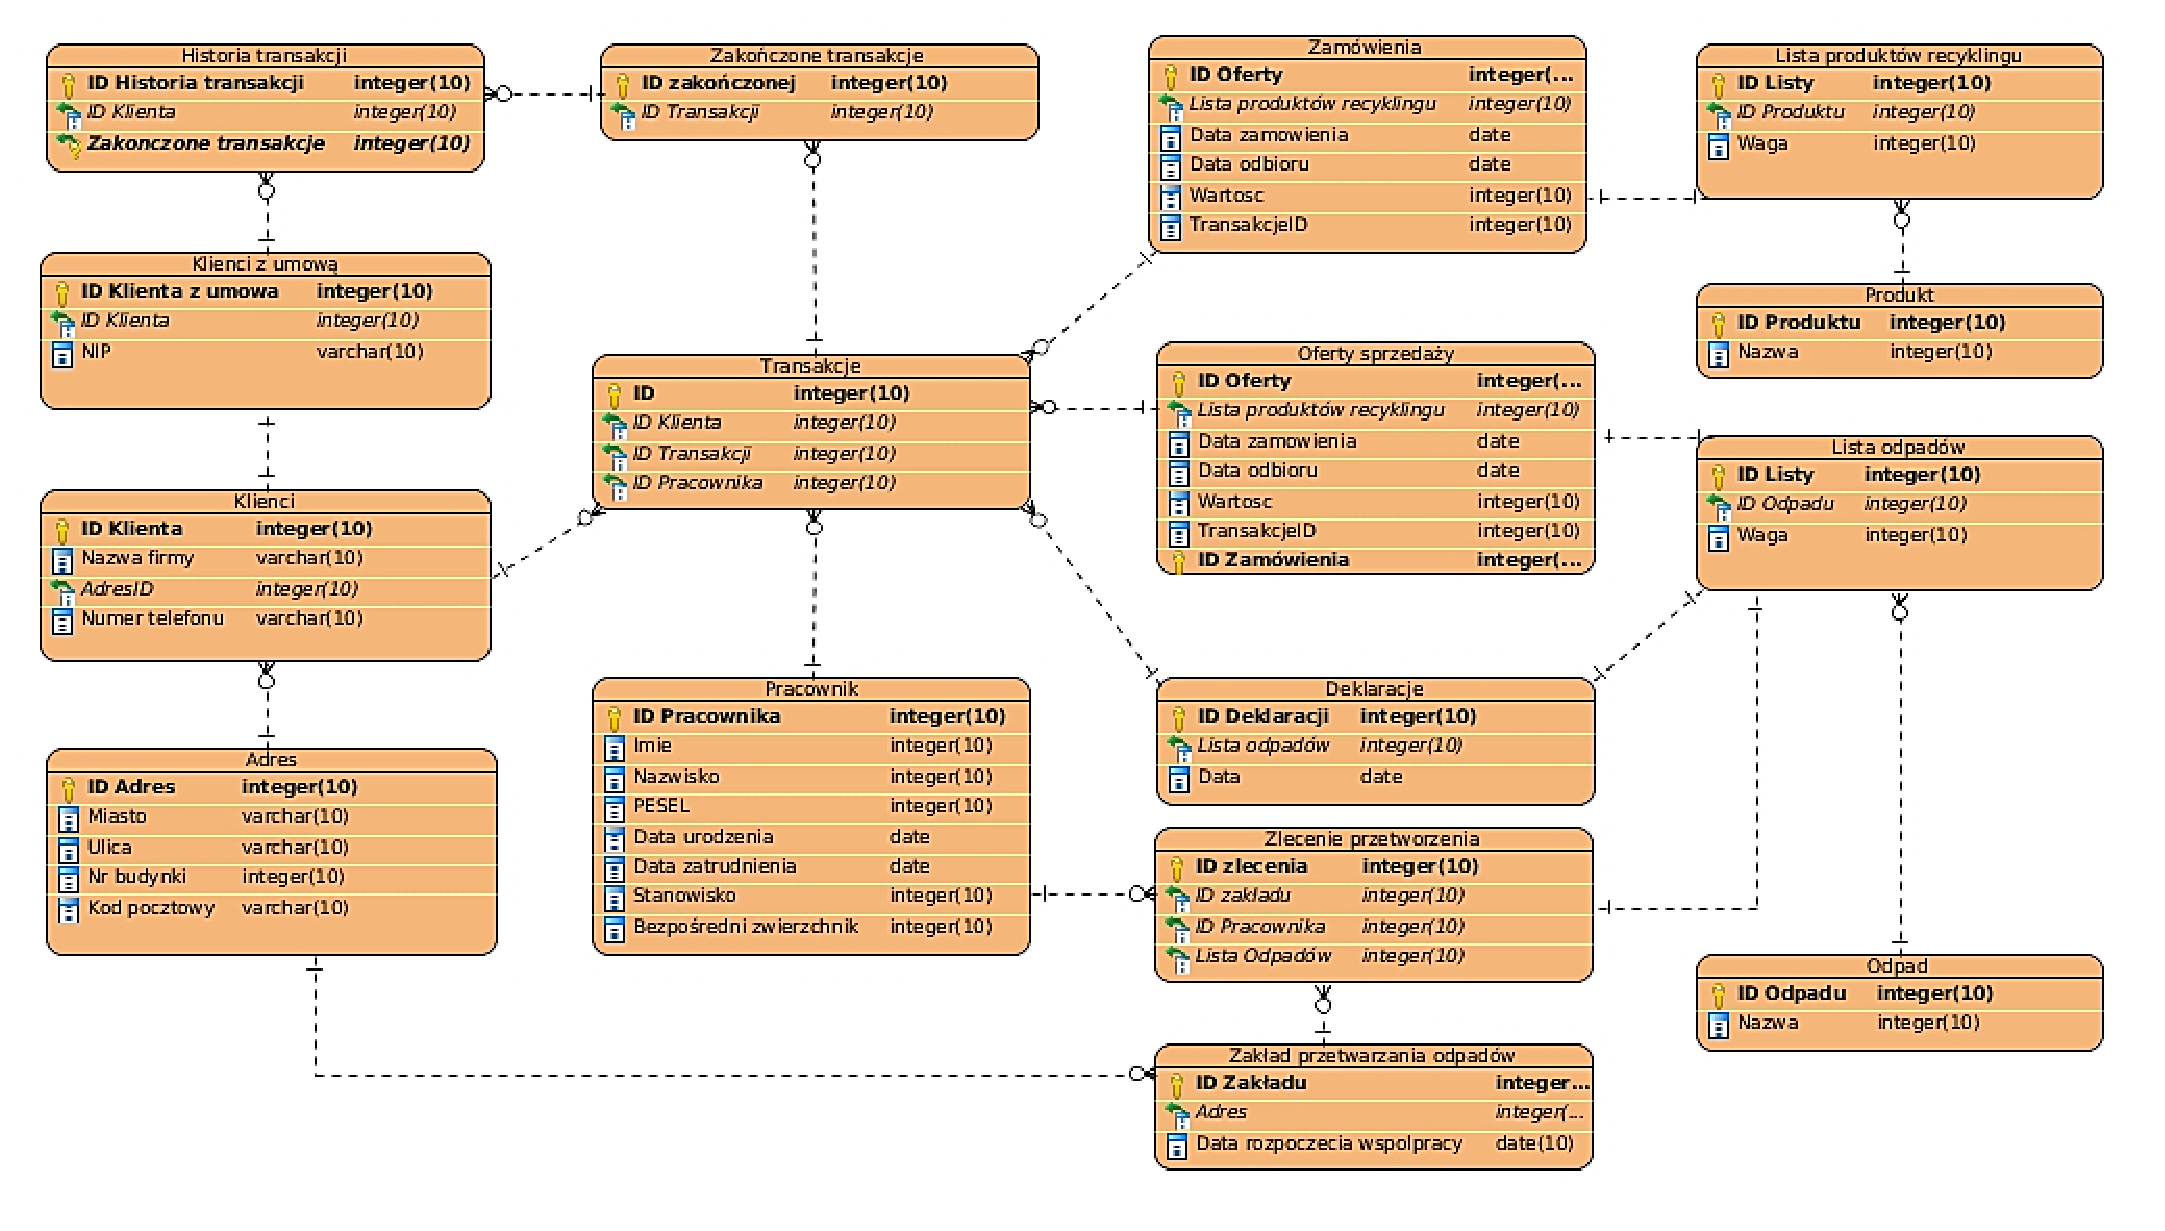
\includegraphics[angle=90, height=29cm]{img/ERD.eps}}
\end{figure}

\textbf{5.3 Opis relacji w tabeli krzyżowej}\\
\begin{table}[h]
\centering
\resizebox{\textwidth}{!}{%
\begin{tabular}{|c|c|c|c|c|c|c|c|c|c|c|}
\hline
                    & Klienci & Klienci z umową & Adres & Historia transakcji & Pracownik & Oferty sprzedaży & Zamówienia & Deklaracje & Odpady & Produkty \\ \hline
Klienci             &         & X               & X     &                     &           & X                & X          & X          &        &          \\ \hline
Klienci z umową     & X       &                 &       & X                   &           & X                & X          & X          &        &          \\ \hline
Adres               & X       &                 &       &                     &           &                  &            &            &        &          \\ \hline
Historia negocjacji &         & X               &       &                     &           & X                & X          & X          &        &          \\ \hline
Pracownik           &         &                 &       &                     &           & X                & X          & X          &        &          \\ \hline
Oferty sprzedaży    & X       & X               &       & X                   & X         &                  &            &            &        & X        \\ \hline
Zamówienia          & X       & X               &       & X                   & X         &                  &            &            & X      &          \\ \hline
Deklaracje          & X       & X               &       & X                   & X         &                  &            &            & X      &          \\ \hline
Odpady              &         &                 &       &                     &           &                  &            &            &        &          \\ \hline
Produkty            &         &                 &       &                     &           &                  &            &            &        &          \\ \hline
\end{tabular}
}
\end{table}